\documentclass[11pt,a4paper]{article}

\usepackage[a4paper,left=18mm,right=18mm,top=17mm,bottom=17mm]{geometry}
\usepackage{helvet}
\usepackage{array}
\usepackage{amsmath}
\usepackage{amssymb}
\usepackage{enumitem}
\usepackage{fancyhdr}
\usepackage{graphicx}
\usepackage{lastpage}
\usepackage{tikz}
\usepackage{xcolor}

\renewcommand{\familydefault}{\sfdefault}
\setlength{\parindent}{0pt}
\setlength{\parskip}{0pt}
\setlength{\headheight}{15pt}
\pagestyle{fancy}
\fancyhf{}
\renewcommand{\headrulewidth}{0pt}
\renewcommand{\footrulewidth}{0pt}

\newcommand{\examtitle}{PHYSICS}
\newcommand{\examcode}{0625/42}
\newcommand{\papername}{Paper 4 Theory (Extended)}
\newcommand{\examseason}{Practice Paper}
\newcommand{\examtime}{1 hour 15 minutes}
\newcommand{\exammarks}{80}
\newcommand{\examyear}{2026}
\newcommand{\examfooter}{0625/42/PRACTICE}
\newcommand{\copyrightline}{\copyright\ Practice paper}

\fancyhead[C]{\ifnum\value{page}>1\textbf{\thepage}\fi}
\fancyfoot[L]{\ifnum\value{page}>1{\small \copyright\ Practice paper}\fi}
\fancyfoot[C]{\ifnum\value{page}>1{\small \examfooter}\fi}
\fancyfoot[R]{\ifnum\value{page}>1\ifodd\value{page}{\small [Turn over}\fi\fi}

\newcommand{\candidateboxes}[1]{%
  \begin{tikzpicture}[baseline=(boxbase.base),x=1mm,y=1mm]
    \node[inner sep=0pt,outer sep=0pt] (boxbase) at (0,6.25) {};
    \foreach \x in {0,...,#1} {
      \draw (\x*8.5,0) -- (\x*8.5,12.5);
    }
    \draw (0,0) rectangle (#1*8.5,12.5);
  \end{tikzpicture}%
}

\newcommand{\namebox}{\fbox{\rule{0pt}{12mm}\hspace{139mm}}}
\newcommand{\candidateentry}[2]{%
  \begin{tabular}[t]{@{}m{24mm}@{}m{45mm}@{}}
    \begin{tabular}{@{}l@{}}#1\\NUMBER\end{tabular} & #2
  \end{tabular}%
}
\newcommand{\nameentry}{%
  \begin{tabular}{@{}m{25mm}@{}m{\dimexpr\linewidth-25mm\relax}@{}}
    \begin{tabular}{@{}l@{}}CANDIDATE\\NAME\end{tabular} & \namebox
  \end{tabular}%
}

\newcommand{\frontpage}{%
  \thispagestyle{empty}
  \vspace*{-7mm}
  \begin{flushright}
    \begin{tabular}{@{}c@{\hspace{2mm}}l@{}}
      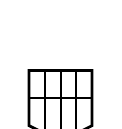
\begin{tikzpicture}[x=1mm,y=1mm,baseline=5mm]
        \draw[line width=0.35mm] (0,9) -- (8,9) -- (8,2) -- (4,0) -- (0,2) -- cycle;
        \draw[line width=0.25mm] (4,9) -- (4,0);
        \draw[line width=0.25mm] (0,5.5) -- (8,5.5);
        \draw[line width=0.25mm] (2,9) -- (2,1);
        \draw[line width=0.25mm] (6,9) -- (6,1);
      \end{tikzpicture} &
      \begin{tabular}{@{}l@{}}
        {\huge\bfseries Cambridge Assessment}\\[-1mm]
        {\huge International Education}
      \end{tabular}
    \end{tabular}
  \end{flushright}

  \vspace{7mm}
  {\Huge\bfseries Cambridge IGCSE\textsuperscript{TM}}\par

  \vspace{7mm}
  \nameentry

  \vspace{3mm}
  \begin{tabular*}{\linewidth}{@{}l@{\extracolsep{\fill}}l@{}}
    \candidateentry{CENTRE}{\candidateboxes{5}} &
    \candidateentry{CANDIDATE}{\candidateboxes{4}}
  \end{tabular*}

  \vspace{4mm}
  \hrule
  \vspace{2mm}
  \small
  \begin{tabular*}{\linewidth}{@{}l@{\extracolsep{\fill}}r@{}}
    {\bfseries \examtitle} & {\bfseries \examcode}\\[2mm]
    \papername & {\bfseries \examseason}\\[2mm]
    & {\bfseries \examtime}
  \end{tabular*}

  \vspace{5.5mm}
  You must answer on the question paper.

  \vspace{4mm}
  No additional materials are needed.

  \vspace{3.5mm}
  \hrule
  \vspace{2mm}
  {\bfseries INSTRUCTIONS}
  \begin{itemize}[leftmargin=5mm,itemsep=0mm,topsep=0.5mm,parsep=0mm,partopsep=0mm]
    \item Answer \textbf{all} questions.
    \item Use a black or dark blue pen. You may use an HB pencil for any diagrams or graphs.
    \item Write your name, centre number and candidate number in the boxes at the top of the page.
    \item Write your answer to each question in the space provided.
    \item Do \textbf{not} use an erasable pen or correction fluid.
    \item Do \textbf{not} write on any bar codes.
    \item You may use a calculator.
    \item You should show all your working and use appropriate units.
    \item Take the weight of 1.0 kg to be 10 N (acceleration of free fall = 10 m/s\textsuperscript{2}).
  \end{itemize}

  \vspace{7mm}
  {\bfseries INFORMATION}
  \begin{itemize}[leftmargin=5mm,itemsep=0mm,topsep=0.5mm,parsep=0mm,partopsep=0mm]
    \item The total mark for this paper is \exammarks.
    \item The number of marks for each question or part question is shown in brackets [\hspace{2mm}].
  \end{itemize}

  \vfill
  \hrule
  \vspace{2mm}
  \begin{center}
    This document has \pageref{LastPage} pages. Any blank pages are indicated.
  \end{center}
  \vspace{5mm}
  \begin{tabular*}{\linewidth}{@{}l@{\extracolsep{\fill}}r@{}}
    DC (PRACTICE) 000000/1 & {\bfseries [Turn over}\\[4mm]
    \copyrightline &
  \end{tabular*}
  \newpage
}

\newcounter{question}
\newcounter{figureinquestion}[question]
\renewcommand{\thefigureinquestion}{\thequestion.\arabic{figureinquestion}}
\newlength{\qnumberwidth}
\newlength{\partlabelwidth}
\newlength{\subpartlabelwidth}
\newlength{\questiontextwidth}
\newlength{\parttextwidth}
\setlength{\qnumberwidth}{8mm}
\setlength{\partlabelwidth}{8mm}
\setlength{\subpartlabelwidth}{8mm}
\setlength{\questiontextwidth}{\dimexpr\textwidth-\qnumberwidth\relax}
\setlength{\parttextwidth}{\dimexpr\textwidth-\qnumberwidth-\partlabelwidth\relax}
\newcolumntype{L}[1]{>{\arraybackslash}p{#1}}
\newcolumntype{P}[1]{>{\arraybackslash}p{#1}}

\newcommand{\question}[2]{%
  \refstepcounter{question}
  \vspace{2mm}
  \begin{tabular}{@{}L{\qnumberwidth}@{}L{\questiontextwidth}@{}}
    \textbf{\thequestion} & #1
  \end{tabular}
  \par\vspace{2mm}
  \def\questiontotal{#2}
}

\newcommand{\questionpart}[3]{%
  \refstepcounter{question}
  \vspace{2mm}
  \begin{tabular}{@{}L{\qnumberwidth}@{}L{\partlabelwidth}@{}L{\parttextwidth}@{}}
    \textbf{\thequestion} & \partlabel{#1} & #2
  \end{tabular}
  \par\vspace{2mm}
  \def\questiontotal{#3}
}

\newcommand{\qtext}[1]{%
  \par\vspace{2mm}
  \begin{tabular}{@{}L{\qnumberwidth}@{}L{\questiontextwidth}@{}}
    & #1
  \end{tabular}
  \par
}

\newcommand{\totalmarks}{%
  \par\vspace{1mm}\hfill [Total: \questiontotal]\par
}

\newcommand{\partlabel}[1]{\textbf{(#1)}}
\newcommand{\subpartlabel}[1]{\textbf{(#1)}}

\newcommand{\partquestion}[2]{%
  \par\vspace{2.5mm}
  \begin{tabular}{@{}L{\qnumberwidth}@{}L{\partlabelwidth}@{}L{\parttextwidth}@{}}
    & \partlabel{#1} & #2
  \end{tabular}
  \par\vspace{1.5mm}
}

\newcommand{\parttext}[1]{%
  \par\vspace{1.5mm}
  \begin{tabular}{@{}L{\qnumberwidth}@{}L{\partlabelwidth}@{}L{\parttextwidth}@{}}
    & & #1
  \end{tabular}
  \par
}

\newcommand{\partsubquestion}[3]{%
  \par\vspace{2.5mm}
  \begin{tabular}{@{}L{\qnumberwidth}@{}L{\partlabelwidth}@{}L{\subpartlabelwidth}@{}L{\dimexpr\parttextwidth-\subpartlabelwidth\relax}@{}}
    & \partlabel{#1} & \subpartlabel{#2} & #3
  \end{tabular}
  \par\vspace{1.5mm}
}

\newcommand{\subpartquestion}[2]{%
  \par\vspace{1.5mm}
  \begin{tabular}{@{}L{\qnumberwidth}@{}L{\partlabelwidth}@{}L{\subpartlabelwidth}@{}L{\dimexpr\parttextwidth-\subpartlabelwidth\relax}@{}}
    & & \subpartlabel{#1} & #2
  \end{tabular}
  \par\vspace{1.5mm}
}

\newcommand{\subparttext}[1]{%
  \par\vspace{1.5mm}
  \begin{tabular}{@{}L{\qnumberwidth}@{}L{\partlabelwidth}@{}L{\subpartlabelwidth}@{}L{\dimexpr\parttextwidth-\subpartlabelwidth\relax}@{}}
    & & & #1
  \end{tabular}
  \par
}

\newcommand{\working}[1][24mm]{\vspace{#1}}

\newcommand{\answerline}[1][110mm]{%
  \makebox[#1]{\leaders\hbox to 0.45em{\hss\raisebox{-0.45ex}{.}\hss}\hfill\kern0pt}
}

\newcommand{\answer}[4][70mm]{%
  \par\hfill #2 = \answerline[#1]\ #3\ [#4]\par
}

\newcommand{\rightanswerline}[2][70mm]{%
  \par\vspace{2mm}
  \hfill #2\ \answerline[#1]\par
}

\newcommand{\rightanswermark}[1]{%
  \par\vspace{-1mm}\hfill [#1]\par
}

\newcommand{\rightanswer}[3][70mm]{%
  \rightanswerline[#1]{#2}%
  \rightanswermark{#3}%
  \par
}

\newcommand{\marksright}[1]{\hfill [#1]\par}

\newcommand{\markinline}[1]{\hfill [#1]}

\newcommand{\writtenanswer}[3][\dimexpr\linewidth-\qnumberwidth-\partlabelwidth-10mm\relax]{%
  \par\vspace{1mm}
  \noindent\hspace*{\dimexpr\qnumberwidth+\partlabelwidth\relax}#2\answerline[#1]\ [#3]%
  \par
}

\newcommand{\writtenline}[2][\dimexpr\linewidth-\qnumberwidth-\partlabelwidth-2mm\relax]{%
  \par\vspace{1mm}
  \noindent\hspace*{\dimexpr\qnumberwidth+\partlabelwidth\relax}#2\answerline[#1]%
  \par
}

\newcommand{\shortwrittenline}[2][64mm]{%
  \par\vspace{1mm}
  \begin{tabular}{@{}P{\qnumberwidth}@{}P{\partlabelwidth}@{}P{\parttextwidth}@{}}
    & & #2\answerline[#1]
  \end{tabular}
  \par
}

\newcommand{\shortwrittenanswer}[3][64mm]{%
  \par\vspace{1mm}
  \noindent\hspace*{\dimexpr\qnumberwidth+\partlabelwidth\relax}#2\answerline[#1]\hfill [#3]%
  \par
}

\newcommand{\subpartwrittenanswer}[3][\dimexpr\linewidth-\qnumberwidth-\partlabelwidth-\subpartlabelwidth-10mm\relax]{%
  \par\vspace{1mm}
  \noindent\hspace*{\dimexpr\qnumberwidth+\partlabelwidth+\subpartlabelwidth\relax}#2\answerline[#1]\ [#3]%
  \par
}

\newcommand{\subpartwrittenline}[2][\dimexpr\linewidth-\qnumberwidth-\partlabelwidth-\subpartlabelwidth-2mm\relax]{%
  \par\vspace{1mm}
  \noindent\hspace*{\dimexpr\qnumberwidth+\partlabelwidth+\subpartlabelwidth\relax}#2\answerline[#1]%
  \par
}

\newcommand{\subpartshortwrittenanswer}[3][64mm]{%
  \par\vspace{1mm}
  \noindent\hspace*{\dimexpr\qnumberwidth+\partlabelwidth+\subpartlabelwidth\relax}#2\answerline[#1]\hfill [#3]%
  \par
}

\newcommand{\twowrittenlines}{%
  \par\vspace{1mm}
  \noindent\hspace*{\dimexpr\qnumberwidth+\partlabelwidth\relax}1.\ \answerline[\dimexpr\linewidth-\qnumberwidth-\partlabelwidth-12mm\relax]\par\vspace{4mm}
  \noindent\hspace*{\dimexpr\qnumberwidth+\partlabelwidth\relax}2.\ \answerline[\dimexpr\linewidth-\qnumberwidth-\partlabelwidth-12mm\relax]
  \par
}

\newcommand{\mcquestion}[1]{%
  \refstepcounter{question}
  \par\vspace{4mm}
  \begin{tabular}{@{}L{\qnumberwidth}@{}L{\questiontextwidth}@{}}
    \textbf{\thequestion} & #1
  \end{tabular}
  \par
}

\newcommand{\mcqtext}[1]{%
  \par\vspace{2mm}
  \begin{tabular}{@{}L{\qnumberwidth}@{}L{\questiontextwidth}@{}}
    & #1
  \end{tabular}
  \par
}

\newcommand{\mcqcenter}[1]{%
  \par\vspace{2mm}
  \noindent\hspace*{\qnumberwidth}%
  \begin{minipage}{\questiontextwidth}
    \centering #1
  \end{minipage}
  \par
}

\newcommand{\mcqimage}[2][\questiontextwidth]{%
  \mcqcenter{\includegraphics[width=#1]{#2}}%
}

\newcommand{\mcqchoices}[4]{%
  \par\vspace{2mm}
  \noindent\hspace*{\qnumberwidth}%
  \begin{tabular}{@{}P{8mm}@{}P{\dimexpr\questiontextwidth-8mm\relax}@{}}
    \textbf{A} & #1\\[1.5mm]
    \textbf{B} & #2\\[1.5mm]
    \textbf{C} & #3\\[1.5mm]
    \textbf{D} & #4
  \end{tabular}
  \par
}

\newcommand{\mcqchoiceswide}[4]{%
  \par\vspace{2mm}
  \noindent\hspace*{\qnumberwidth}%
  \begin{tabular*}{\questiontextwidth}{@{}l@{\extracolsep{\fill}}l@{\extracolsep{\fill}}l@{\extracolsep{\fill}}l@{}}
    \textbf{A}\quad #1 & \textbf{B}\quad #2 & \textbf{C}\quad #3 & \textbf{D}\quad #4
  \end{tabular*}
  \par
}

\newcommand{\mcqchoicegrid}[4]{%
  \par\vspace{2mm}
  \noindent\hspace*{\qnumberwidth}%
  \begin{tabular*}{\questiontextwidth}{@{}c@{\extracolsep{\fill}}c@{}}
    \textbf{A}\\[1mm]#1 & \textbf{B}\\[1mm]#2\\[5mm]
    \textbf{C}\\[1mm]#3 & \textbf{D}\\[1mm]#4
  \end{tabular*}
  \par
}

\newenvironment{mcqtable}[1]{%
  \par\vspace{2mm}
  \noindent\hspace*{\qnumberwidth}%
  \renewcommand{\arraystretch}{1.35}%
  \begin{tabular}{#1}
}{%
  \end{tabular}
  \par
}

\newcommand{\answerbox}[1][28mm]{%
  \begin{center}
    \fbox{\begin{minipage}{\parttextwidth}\vspace{#1}\end{minipage}}
  \end{center}
}

\newcommand{\figref}[1]{\ref{#1}}

\newcommand{\maybefiglabel}[1]{%
  \if\relax\detokenize{#1}\relax
  \else
    \label{#1}%
  \fi
}

\newcommand{\examfigure}[2]{%
  \refstepcounter{figureinquestion}%
  \begin{center}
    #2\\[1mm]
    {\bfseries Fig. \thefigureinquestion}%
    \maybefiglabel{#1}%
  \end{center}
}

\newcommand{\figplaceholder}[3][]{%
  \examfigure{#1}{%
    \begin{tikzpicture}
      \draw[gray!70] (0,0) rectangle (#2,#3);
      \draw[gray!70] (0,0) -- (#2,#3);
      \draw[gray!70] (0,#3) -- (#2,0);
      \node[gray!70] at (#2/2,#3/2) {diagram area};
    \end{tikzpicture}%
  }%
}

\newcommand{\blankpage}{%
  \newpage
  \thispagestyle{fancy}
  \vspace*{\fill}
  \begin{center}
    \textbf{BLANK PAGE}
  \end{center}
  \vspace*{\fill}
  \newpage
}

\begin{document}

\frontpage

\mcquestion{Which instrument is most suitable to determine the volume of a small irregularly shaped stone?}
\mcqchoices
  {30 cm ruler}
  {digital timer}
  {measuring cylinder}
  {tape measure}

\mcquestion{A steel ball is dropped from the top floor of a building. Air resistance can be ignored.}
\mcqtext{Which statement describes the motion of the ball?}
\mcqchoices
  {The ball falls with constant acceleration.}
  {The ball falls with constant speed.}
  {The ball falls with decreasing speed.}
  {The ball falls with increasing acceleration.}

\mcquestion{The diagram shows a velocity-time graph for an object which is accelerating.}
\mcqimage[82mm]{assets/mcq/q03_velocity_time_graph.png}
\mcqtext{What is the acceleration of the object?}
\mcqchoiceswide
  {0.40 m/s\textsuperscript{2}}
  {2.5 m/s\textsuperscript{2}}
  {3.0 m/s\textsuperscript{2}}
  {100 m/s\textsuperscript{2}}

\newpage

\mcquestion{Diagram 1 shows a piece of flexible material that contains many pockets of air. Diagram 2 shows the same piece of flexible material after it has been compressed so that its volume decreases.}
\mcqimage[105mm]{assets/mcq/q04_compression_diagrams.png}
\mcqtext{What happens to the mass and to the weight of the flexible material when it is compressed?}
\begin{mcqtable}{|c|c|c|}
\hline
 & mass & weight \\ \hline
\textbf{A} & increases & increases \\ \hline
\textbf{B} & increases & no change \\ \hline
\textbf{C} & no change & increases \\ \hline
\textbf{D} & no change & no change \\ \hline
\end{mcqtable}

\mcquestion{A student determines the density of copper. She has a rectangular block of copper.}
\mcqtext{Which other apparatus does she need?}
\begin{mcqtable}{|c|c|c|c|c|}
\hline
 & balance & ruler & stop-watch & thermometer \\ \hline
\textbf{A} & \checkmark & \checkmark & \checkmark & \checkmark \\ \hline
\textbf{B} & \checkmark & \checkmark & \checkmark & \textit{x} \\ \hline
\textbf{C} & \checkmark & \checkmark & \textit{x} & \textit{x} \\ \hline
\textbf{D} & \checkmark & \textit{x} & \textit{x} & \textit{x} \\ \hline
\end{mcqtable}

\mcquestion{A 0.15 kg mass is suspended from a vertical spring. The mass is pulled downwards until the spring has extended by 12 cm from its unstretched length.}
\mcqtext{The spring constant of the spring is 30 N/m. What is the magnitude of the initial acceleration of the spring when it is released?}
\mcqchoiceswide
  {14 m/s\textsuperscript{2}}
  {24 m/s\textsuperscript{2}}
  {28 m/s\textsuperscript{2}}
  {34 m/s\textsuperscript{2}}

\newpage

\mcquestion{A cricket ball of mass 0.15 kg is moving at a speed of 30 m/s.}
\mcqtext{The diagram shows a batsman holding a bat stationary as the ball hits the bat and bounces back at the same speed in the opposite direction.}
\mcqimage[90mm]{assets/mcq/q07_cricket_bat.png}
\mcqtext{The ball is in contact with the bat for $1.0 \times 10^{-3}$ s. Which row is correct?}
\begin{mcqtable}{|c|c|c|}
\hline
 & \begin{tabular}{c}change of momentum\\kg m/s\end{tabular} & force applied to ball / N \\ \hline
\textbf{A} & 4.5 & 4500 \\ \hline
\textbf{B} & 4.5 & 9000 \\ \hline
\textbf{C} & 9.0 & 4500 \\ \hline
\textbf{D} & 9.0 & 9000 \\ \hline
\end{mcqtable}

\mcquestion{A stone is thrown vertically upwards at a speed of 5.0 m/s.}
\mcqtext{All of the energy initially in the kinetic store of the stone is transferred to its gravitational potential store when the stone reaches its maximum height. Which equation gives the maximum height $h$ reached by the stone?}
\mcqchoices
  {$h=\dfrac{9.8}{2 \times 5.0^2}$}
  {$h=\dfrac{5.0^2 \times 2}{9.8}$}
  {$h=\dfrac{5.0^2}{2 \times 9.8}$}
  {$h=\dfrac{2 \times 9.8}{5.0^2}$}

\newpage

\mcquestion{Which wave will diffract the most when passing through a gap that is 0.85 m wide?}
\begin{mcqtable}{|c|c|c|}
\hline
 & \begin{tabular}{c}wave speed\\m/s\end{tabular} & wave frequency / Hz \\ \hline
\textbf{A} & 300 & 280 \\ \hline
\textbf{B} & 300 & 400 \\ \hline
\textbf{C} & 350 & 280 \\ \hline
\textbf{D} & 350 & 400 \\ \hline
\end{mcqtable}

\mcquestion{Which arrow on the graph shows the amplitude of the wave?}
\mcqimage[110mm]{assets/mcq/q18_wave_amplitude.png}

\mcquestion{Which row describes a seismic S-wave?}
\begin{mcqtable}{|c|p{30mm}|p{92mm}|}
\hline
 & type of wave & direction of vibration \\ \hline
\textbf{A} & longitudinal & parallel to the direction of travel of the wavefront \\ \hline
\textbf{B} & longitudinal & perpendicular to the direction of travel of the wavefront \\ \hline
\textbf{C} & transverse & parallel to the direction of travel of the wavefront \\ \hline
\textbf{D} & transverse & perpendicular to the direction of travel of the wavefront \\ \hline
\end{mcqtable}

\newpage

\mcquestion{A ray of light, travelling in air, is incident on an air-glass boundary.}
\mcqtext{The angles between the incident ray, the refracted ray and the boundary are shown.}
\mcqimage[70mm]{assets/mcq/q21_refraction.png}
\mcqtext{Which equation is used to calculate the refractive index $n$ of the glass?}
\mcqchoiceswide
  {$n=\dfrac{\sin40^\circ}{\sin26^\circ}$}
  {$n=\dfrac{\sin40^\circ}{\sin64^\circ}$}
  {$n=\dfrac{\sin50^\circ}{\sin26^\circ}$}
  {$n=\dfrac{\sin50^\circ}{\sin64^\circ}$}

\mcquestion{A small object O is placed near a converging lens, as shown. The lens forms an image I.}
\mcqimage[95mm]{assets/mcq/q22_lens_image.png}
\mcqtext{Which statement is correct?}
\mcqchoices
  {The image I is diminished.}
  {The image I is inverted.}
  {The image I is real.}
  {The object O is closer to the lens than its principal focus.}

\newpage

\mcquestion{A metallic wire X has a resistance.}
\mcqtext{What is the difference in resistance for a wire of the same material as X that is shorter than X but the same diameter, and for a wire that has the same length as X but a smaller diameter?}
\begin{mcqtable}{|c|p{42mm}|p{48mm}|}
\hline
 & resistance of shorter wire & resistance of wire with smaller diameter \\ \hline
\textbf{A} & greater & greater \\ \hline
\textbf{B} & greater & smaller \\ \hline
\textbf{C} & smaller & greater \\ \hline
\textbf{D} & smaller & smaller \\ \hline
\end{mcqtable}

\mcquestion{The diagram shows the circuit for a potential divider.}
\mcqimage[56mm]{assets/mcq/q29_potential_divider.png}
\mcqtext{Which equation is used to calculate $V_1$?}
\mcqchoices
  {$V_1=\dfrac{R_1}{V_2 \times (R_1+R_2)}$}
  {$V_1=\dfrac{V_2 \times R_1}{R_2}$}
  {$V_1=\dfrac{V_2 \times R_1}{R_1+R_2}$}
  {$V_1=\dfrac{R_1}{V_2 \times R_2}$}

\newpage

\mcquestion{When there is an electric current in a long straight wire, a magnetic field is created around the wire.}
\mcqtext{Which diagram shows the correct pattern and direction of magnetic field lines around a long straight wire carrying current into the page?}
\mcqimage[118mm]{assets/mcq/q32_magnetic_field_choices.png}

\mcquestion{When a thin gold foil is bombarded with alpha particles, some alpha particles are deflected through large angles.}
\mcqtext{Which statement explains this deflection?}
\mcqchoices
  {Most of the atom consists of empty space.}
  {All of the positive charge and most of the mass of the gold atom are concentrated in a small volume.}
  {Positive charge in the gold atom is spread evenly throughout the atom.}
  {All of the negative charge is concentrated at its centre.}

% Structured question examples are kept below, but temporarily disabled while
% the Paper 2 multiple-choice workflow is being refined.
\iffalse
\newpage
\setcounter{question}{0}

\question{Fig. \figref{fig:electric-bicycle} shows an electrically powered bicycle.}{8}
\examfigure{fig:electric-bicycle}{%
  \includegraphics[
    page=2,
    trim=35mm 185mm 35mm 26mm,
    clip,
    width=120mm
  ]{0625_s22_qp_42.pdf}%
}

\qtext{The battery can deliver a power of 600 W for 60 min.}

\partsubquestion{a}{i}{Calculate the energy, in joules, stored in the battery when fully charged.}
\working[26mm]
\answer{energy}{J}{3}

\subpartquestion{ii}{State the form of energy stored by the battery.}
\subpartwrittenanswer{ }{1}

\partquestion{b}{The bicycle has a motor with an electrical input power of 250 W.}
\parttext{Calculate the time for which the battery can power the bicycle.}
\working[26mm]
\answer{time}{s}{2}

\partquestion{c}{State two environmental benefits of using an electrically powered bicycle instead of a small motorcycle.}
\twowrittenlines
\marksright{2}
\totalmarks

\newpage

\question{Fig. \figref{fig:pulley-bench} shows two objects connected by a cord passing over a pulley.}{9}
\examfigure{fig:pulley-bench}{%
  \includegraphics[
    page=3,
    trim=48mm 211mm 43mm 36mm,
    clip,
    width=95mm
  ]{0625_s22_qp_42.pdf}%
}

\qtext{The 2.0 kg object is released from rest and accelerates at 4.0 m/s\textsuperscript{2}.}

\partquestion{a}{Calculate the resultant force acting on the 2.0 kg object.}
\working[25mm]
\answer{force}{N}{2}

\partquestion{b}{Calculate the upward force exerted by the cord on the 3.0 kg object.}
\working[28mm]
\answer{force}{N}{3}

\partsubquestion{c}{i}{The objects have a constant acceleration.}
\subparttext{Show that the speed of the objects 0.80 s after release is 3.2 m/s.}
\working[24mm]
\marksright{2}

\subpartquestion{ii}{A card of width 2.0 cm passes through a beam of light at this speed. Calculate the time taken for the card to pass through the beam.}
\working[25mm]
\answer{time}{s}{2}
\totalmarks

\newpage

\questionpart{a}{Fig. \figref{fig:river-canoe} shows water in a river moving parallel to the river bank at 4.0m/s and a canoe travelling in the river.}{8}
\examfigure{fig:river-canoe}{%
  \includegraphics[
    page=4,
    trim=25mm 181mm 25mm 31mm,
    clip,
    width=135mm
  ]{0625_s22_qp_42.pdf}%
}

\parttext{The canoe travels at 2.5m/s relative to the water and heads at an angle of 38\textdegree{} to the river bank.}

\parttext{Draw a scale diagram to determine the canoe's resultant velocity and state the scale you used.}
\working[70mm]
\rightanswerline[80mm]{scale}
\rightanswerline[80mm]{magnitude of resultant velocity}
\rightanswerline[80mm]{direction of resultant velocity (angle from the river bank)}
\rightanswermark{4}

\partquestion{b}{Explain why the resultant velocity is not in the same direction as the canoe points.}
\writtenline{ }
\writtenline{ }
\marksright{2}
\totalmarks

\newpage

\question{A student investigates the resistance of a wire.}{10}
\figplaceholder[fig:resistance-wire]{11}{4.2}

\partquestion{a}{Complete the table headings for the measurements needed in this experiment.}

\begin{center}
\renewcommand{\arraystretch}{1.8}
\begin{tabular}{|p{38mm}|p{38mm}|p{38mm}|}
\hline
\textbf{Length of wire / cm} & & \\ \hline
20 & & \\ \hline
40 & & \\ \hline
60 & & \\ \hline
80 & & \\ \hline
\end{tabular}
\end{center}
\marksright{2}

\partquestion{b}{Describe how the student can use the measurements to determine the resistance of the wire.}
\answerbox[34mm]
\marksright{4}

\partquestion{c}{State two precautions that improve the reliability of the results.}
\twowrittenlines
\marksright{2}

\partquestion{d}{On the grid, sketch the expected shape of a graph of resistance against length for a uniform wire.}
\begin{center}
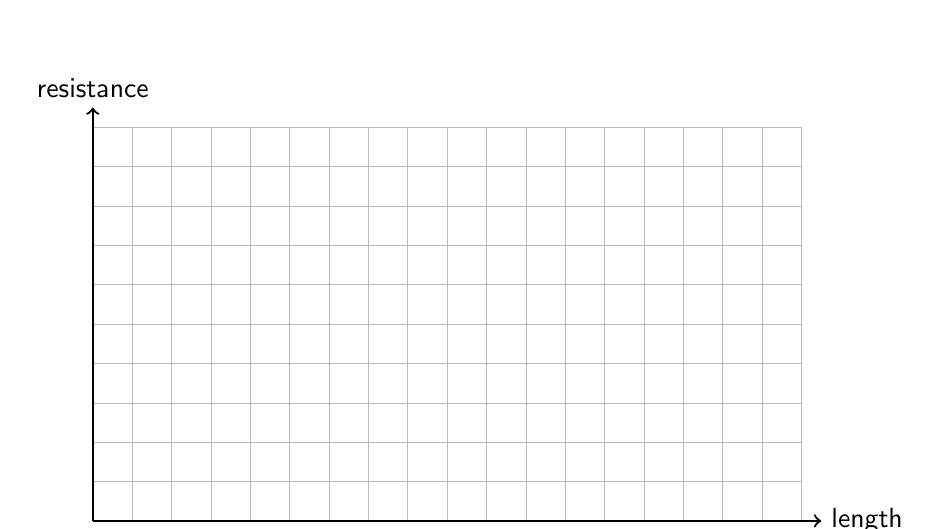
\begin{tikzpicture}[x=0.5cm,y=0.5cm]
  \draw[step=0.5cm,gray!55,very thin] (0,0) grid (18,10);
  \draw[thick,->] (0,0) -- (18.5,0) node[right] {length};
  \draw[thick,->] (0,0) -- (0,10.5) node[above] {resistance};
\end{tikzpicture}
\end{center}
\marksright{2}
\totalmarks

\blankpage

\question{This page shows the structure for adding another long question. Replace this text with your own question stem.}{6}
\partquestion{a}{Write the first part of the question here.}
\working[18mm]
\answer{answer}{unit}{2}
\partquestion{b}{Write the second part of the question here.}
\answerbox[30mm]
\marksright{4}
\totalmarks

\fi

\end{document}
